\subsection{Properties of Functions: Even or Odd}
\begin{definition}[Even]
	Even functions are symmetric about $y$-axes in a graph.
\end{definition}

\begin{example}[Even Function] 
	This is an even function because if we fold it down the $y$-axis and fold it onto itself, it would be a mirror image perfectly.
	$$f(x) = x^2$$
	\hfill
	\begin{center}
	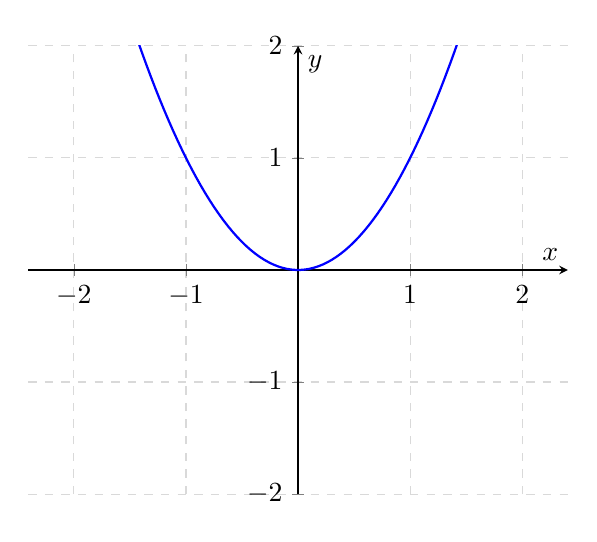
\begin{tikzpicture}
		\begin{axis}[
		    axis lines = center,
		    xlabel = $x$,
		    ylabel = $y$,
		    xmin = -2, xmax = 2,
		    ymin = -2, ymax = 2,
		    grid = both,
		    grid style = {dashed, gray!30},
		    axis equal
		]
		    \addplot [domain=-2:2, samples=100, thick, blue] {x^2};
		\end{axis}
	\end{tikzpicture}
	\end{center}
\end{example}

\begin{definition}[Odd]
	Odd functions are symmetric about origins in a graph.
\end{definition}

\begin{example}[Odd Function] 
	This is an odd function because if we rotate the graph $180^{\circ}$ about the origin, it will still be the exact same graph.
	$$f(x) = x^3 - x$$
	\hfill
	\begin{center}
	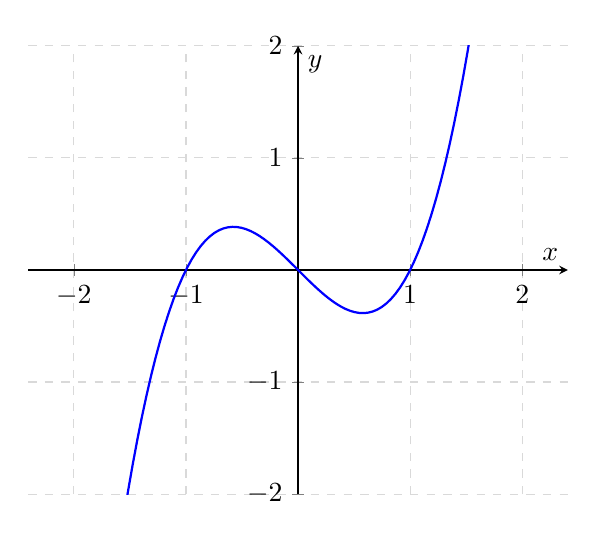
\begin{tikzpicture}
		\begin{axis}[
		    axis lines = center,
		    xlabel = $x$,
		    ylabel = $y$,
		    xmin = -2, xmax = 2,
		    ymin = -2, ymax = 2,
		    grid = both,
		    grid style = {dashed, gray!30},
		    axis equal
		]
		    \addplot [domain=-2:2, samples=100, thick, blue] {x^3 - x};
		\end{axis}
	\end{tikzpicture}
	\end{center}
\end{example}

\newpage
\textbf{Note: }A lot of graphs are neither even or odd. For example:
\begin{example}[Neither]
	$$f(x) = x^2 + x$$
	\hfill
	\begin{center}
	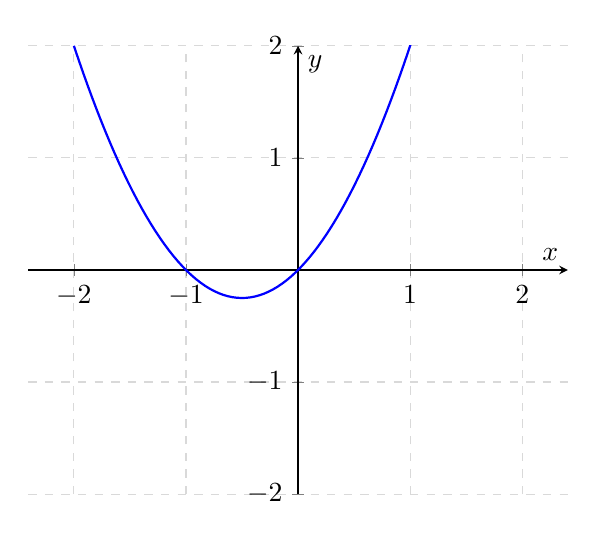
\begin{tikzpicture}
		\begin{axis}[
		    axis lines = center,
		    xlabel = $x$,
		    ylabel = $y$,
		    xmin = -2, xmax = 2,
		    ymin = -2, ymax = 2,
		    grid = both,
		    grid style = {dashed, gray!30},
		    axis equal
		]
		    \addplot [domain=-2:2, samples=100, thick, blue] {x^2 + x};
		\end{axis}
	\end{tikzpicture}
	\end{center}
\end{example}

\begin{definition}[Algebraic Definition of Even Functions]
	$$f(x) = f(-x)$$
\end{definition}

\begin{definition}[Algebraic Definition of Odd Functions]
	$$-f(x) = f(-x)$$
\end{definition}

\begin{example}[Algebraic]
	\hfill
	\begin{itemize}
		\item $f(x) = 2x^4 - x^2$ \\
		$f(-x) = 2(-x)^4 - (-x)^2$ \\
		$f(-x) = 2x^4 - x^2 \quad Even$
		\item $g(x) = \frac{x}{x^2 - 1}$ \\
		$g(-x) = \frac{(-x)^1}{(-x)^2 - 1} \to g(-x) = \frac{-x}{x^2 - 1}$ \\
		$g(-x) = -\frac{x}{x^2 - 1} \quad Odd$
		\item $h(x) = 3x^3 + 5$ \\
		$h(-x) = 3(-x)^3 + 5 \to h(-x) = -3x^3 + 5$ \\
		$h(-x) = -(3x^3 - 5) \quad Neither$
		\item $F(x) = \frac{x^2 + 3}{x^2 - 1}$ \\
		$F(-x) = \frac{(-x)^2 + 3}{(-x)^2 - 1}$ \\
		$F(-x) = \frac{x^2 + 3}{x^2 - 1} \quad Even$
		\item $G(x) = \sqrt{x}$ \\
		$G(-x) = \sqrt{(-x)} \quad Neither\:because\:it's\:not\:a\:\R\:number$ \\
		\item $H(x) = \frac{-x^3}{3x^2 - 9} \to -\frac{x^3}{3x^2 - 9}$ \\
		$H(-x) = \frac{-(-x)^3}{3x^2 - 9}$ \\
		$H(-x) = \frac{x^3}{3x^2 - 9} \quad Odd$
	\end{itemize}
\end{example}
